\part{Les objectifs de ce projet}
    \chapter{Les cas d'usage}
        \section{Objectifs : Qualité et productivité}

        Comme présenté précédemment (cf. \reffig{fig:processus_article}), la gestion de l'information produit est un processus lourd, avec des étapes de contrôle redondantes visant à assurer la qualité de la donnée.
        Un traitement automatique des documents mis à disposition permettrait de décharger les personnes qui interviennent dans le processus (fournisseurs, acheteurs, gestionnaires de référentiels, ingénieurs qualité) et de garantir une meilleure pertinence de l'information produit.

        \section{La préalimentation d'information}
        Une des manières de gagner en productivité et en qualité serait :
        \begin{itemize}
            \item de modifier l'interface homme machine de l'écran de saisie des données par le fournisseur, pour que le chargement des pièces jointes se fasse en premier
            \item d'interpréter le contenu des pièces jointes dès qu'elles sont chargées, pour alimenter les autres champs de saisie
            \item laisser ensuite au fournisseur la possibilité de compléter et corriger ces informations avant de les soumettre à Pomona
        \end{itemize} 
        Il est illusoire d'automatiser totalement la saisie et d'imaginer se passer d'une saisie complémentaire par le fournisseur.
        La mise en place de la GDSN (cf. section \mref{GDSN}), qui permet pourtant de faire transiter par EDI les données produit de manière standardisée et efficace, n'a pas permis de s'affranchir de cette tâche.
        Sous réserve d'avoir un outil suffisamment fiable, on pourrait faire gagner du temps aux fournisseurs et améliorer la qualité de l'information produit.
        Néanmoins, plusieurs freins existent à la mise en place 
        \begin{itemize}
            \item cela n'a d'intérêt que si le système est capable de produire de l'information structurée avec une fiabilité élevée (par exemple, 80\% de données correctes serait un minimum)
            \item cela entre en concurrence directe avec le système GDSN - avec la question de la manière de gérer les conflits entre les information issues de ce réseau et celles extraites des pièces jointes
            \item cela apporte l'essentiel de la valeur aux fournisseurs, et pas au groupe
        \end{itemize}

        \section{Le contrôle des informations transmises}

        Plus le taux de détection des erreurs est élevé, et plus les erreurs sont détectées tôt, mieux c'est : 
        \begin{itemize}
            \item la qualité des données s'en trouve évidemment améliorée
            \item le processus est plus court en temps, en évitant les aller-retours
            \item on décharge l'ensemble des acteurs, en limitant le nombre d'interventions de chacun, ainsi que la charge administrative de synchronisation de leurs actions             
        \end{itemize}
        Les différentes étapes possibles pour lesquelles effectuer un contrôle sont présentées à la \reffig{fig:processus_article_aide_ctrle}.

        \begin{figure}[htbp]
            \begin{center}
            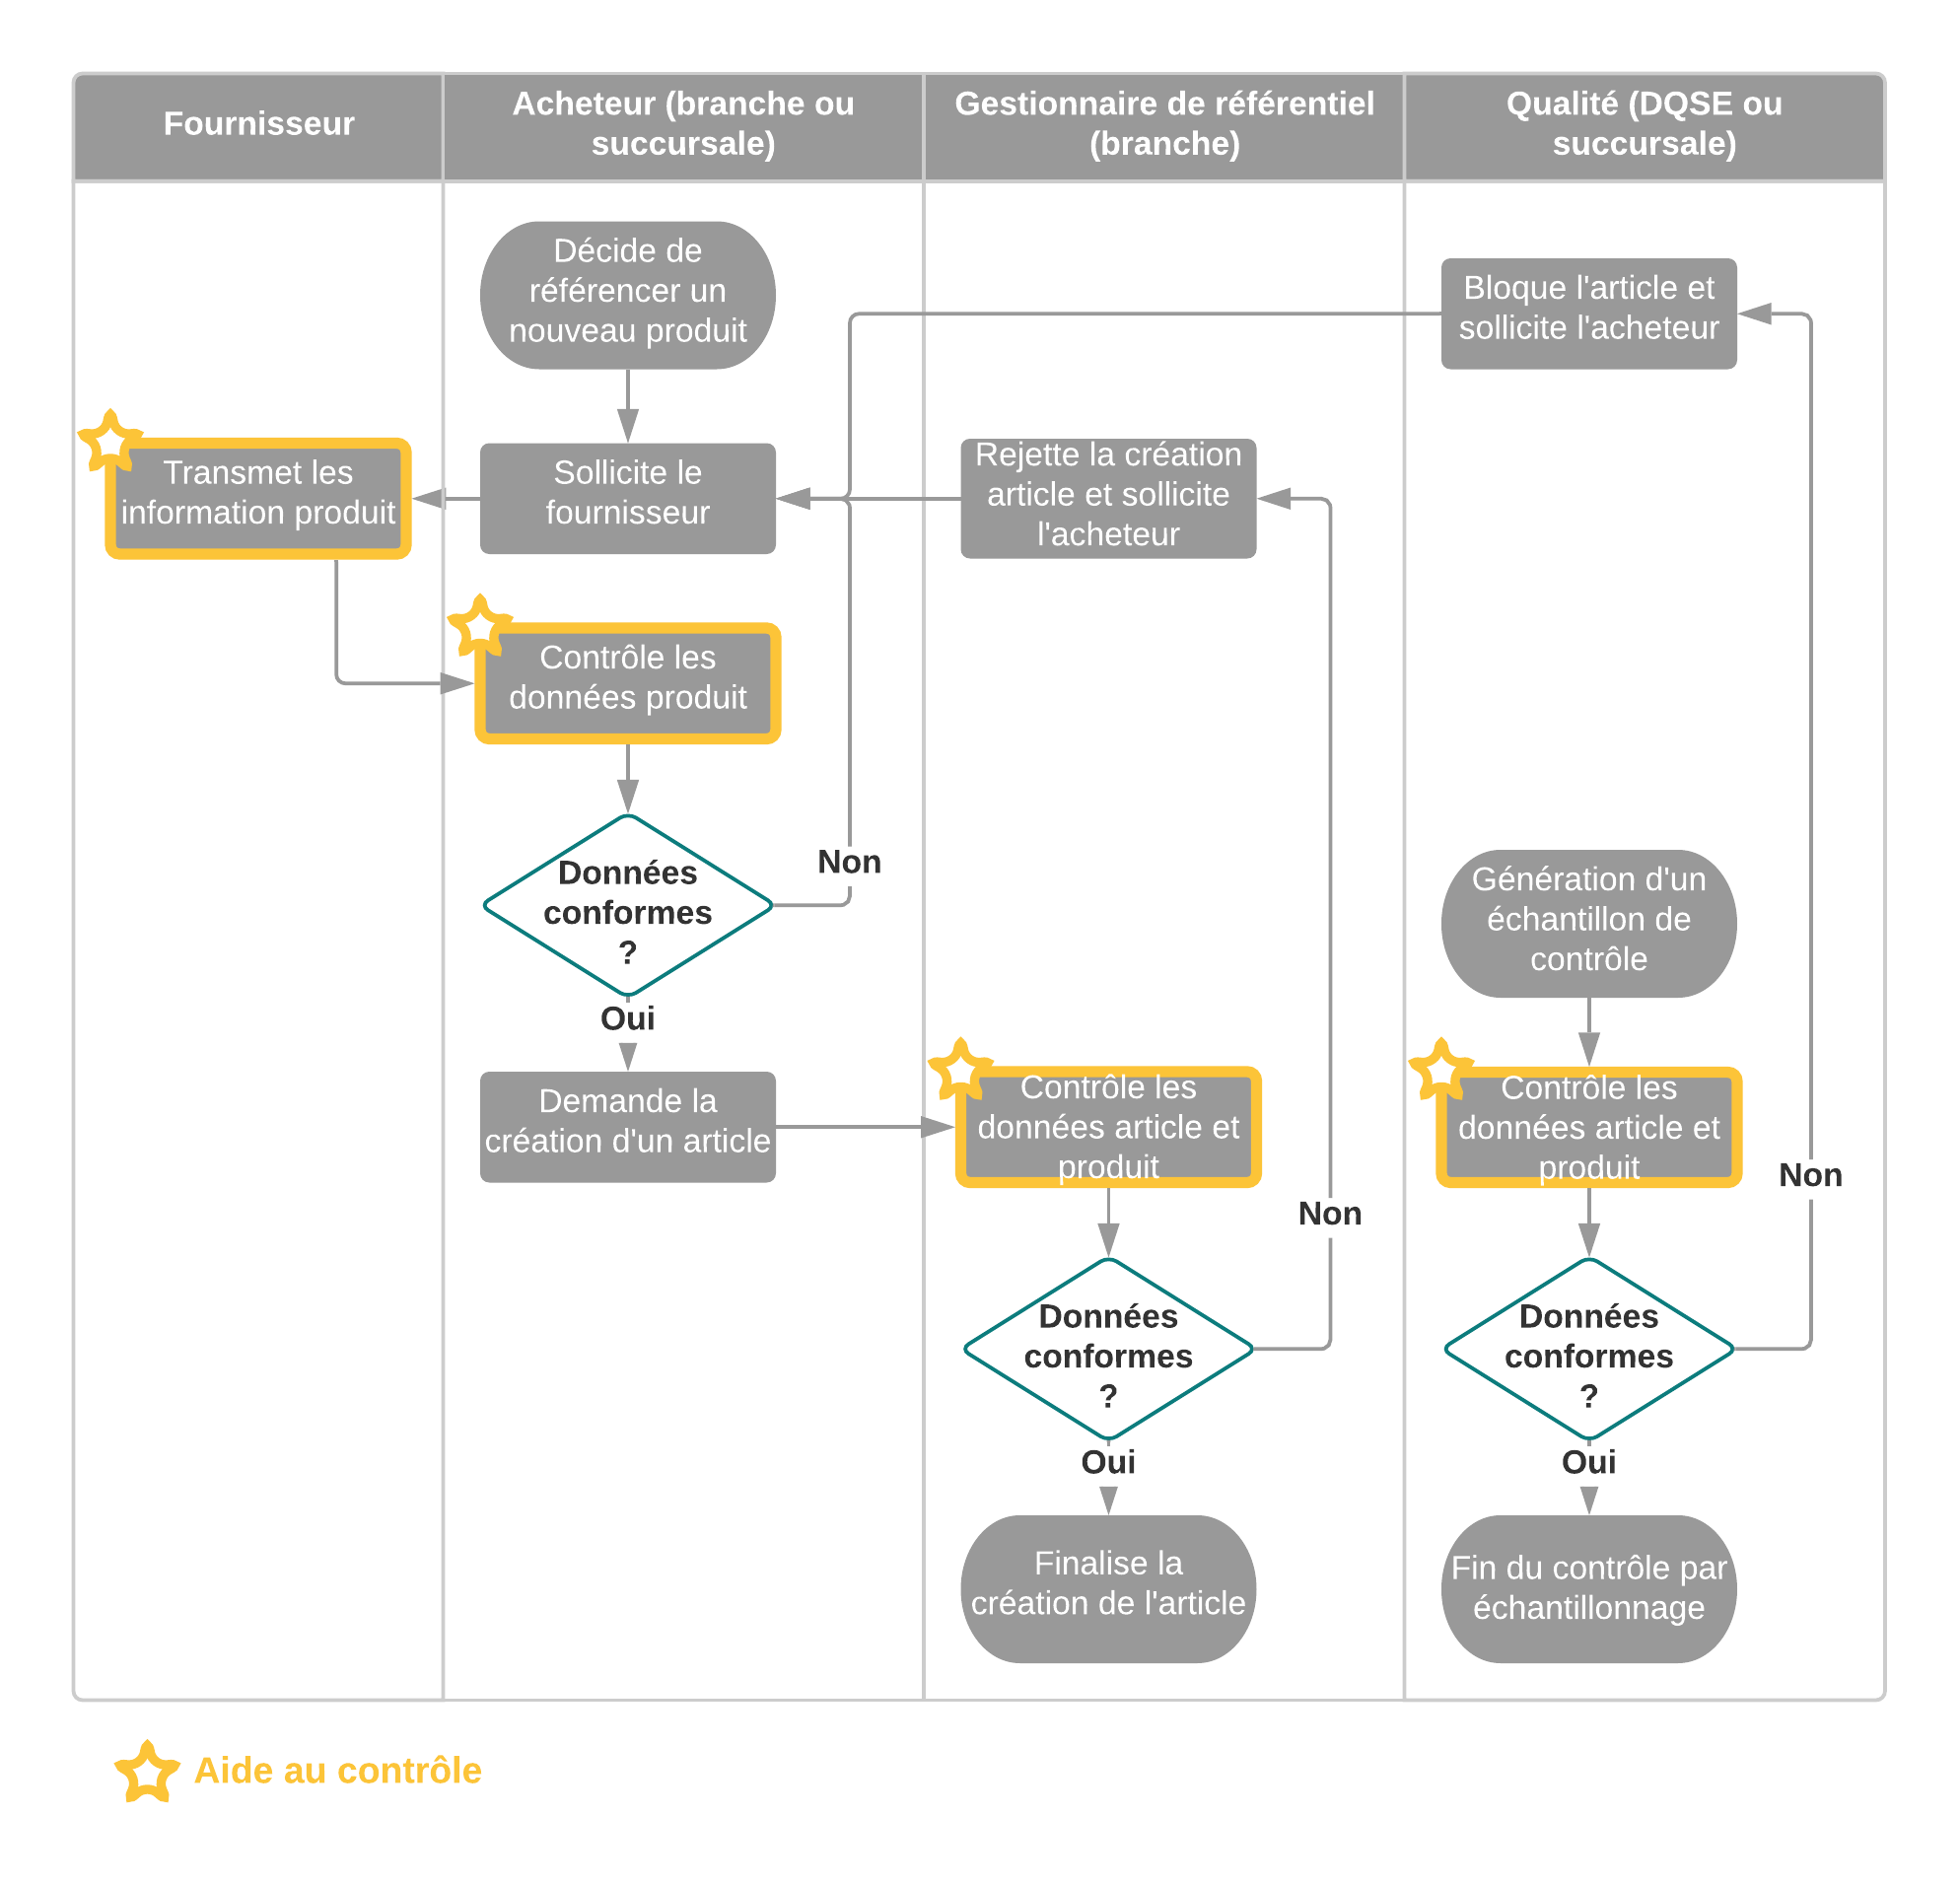
\includegraphics[width=0.9\linewidth]{img/Processus_de_creation_article_avec_aide_au_controle.png}
            \end{center}
            \caption{\'{E}tapes du processus article pouvant être améliorées}
            \label{fig:processus_article_aide_ctrle}
        \end{figure}    

            \subsection{Le contrôle à la saisie fournisseur}
            Si on déclenche un contrôle au moment où le fournisseur soumet les données et qu'on l'alerte en cas d'incohérence, on peut dès le début du processus éviter une erreur.
            L'avantage d'avoir une identification des problèmes aussi tôt est qu'on économise immédiatement au moins une étape de contrôle des données.

            \subsection{L'aide aux vérifications Pomona}
            Lors des contrôles inclus au sein du processus, on pourrait mettre en évidence les incohérences détectées entre pièces jointes et données à contrôler.
            Cela permettrait de fiabiliser les étapes de contrôle, et éviter qu'une erreur soit détectée tardivement (par les gestionnaires de référentiel ou les ingénieurs qualité).
            C'est d'autant plus intéressant que la première étape de contrôle est faite par les acheteurs.
            Dans la mesure où c'est une tâche administrative qui n'est pas dans leur c{\oe}ur de métier, elle est souvent effectuée rapidement et est peu efficace.

            \subsection{Les contrôles en masse asynchrones}
            Enfin, il pourrait être pertinent de faire tourner de manière asynchrone des contrôles de qualité de données sur l'ensemble de la base.
            Il pourrait sembler inutile d'effectuer cette tâche alors qu'on a une validation des données par l'application (contrôles \og informatiques \fg) et par des contrôleurs humains.
            Néanmoins, il arrive fréquemment que des changements de règles de gestion informatiques ou métier soit mis en place, sans que les données soient ensuite remises à jour.
            Par exemple, les mentions des traces d'allergènes dans les ingrédients était par le passé retirées des listes d'ingrédients, alors qu'elle sont aujourd'hui incluses. 
            Mais aucun chantier de remise à niveau de l'historique n'a été entrepris au moment du changement de règle, d'où des données qui ne sont pas alignées avec les règles de gestion.

    \chapter{Le choix du cas d'usage}

        \section{La représentation dominante des fiches techniques}
        On a beaucoup de fiches techniques, pas beaucoup d'étiquettes ou de fiches logistiques (cf. la table qui va bien.)
        On va donc plutôt dans un premier temps tenter de travailler avec les fiches techniques.

        \section{Les multiples formats et le besoin de \og spatialisation \fg}
        \label{formats_spatialisation}

        Chaque fournisseur décide évidemment du format de document qu'il souhaite produire.
        On a donc beaucoup de formats différents, et un Pareto finalement trop \og mou \fg pour envisager de construire des templates pour récupérer les informations automatiquement (cf. \reffig{fig:rappel_pdt_par_frn}).
    
        \section{Les informations \og spatialisées \fg}
        Les données que l'on souhaite récupérer sont globalement de 3 types : 
        \begin{itemize}
            \item données de composition
            \item données nutritionnelles
            \item données logistiques
        \end{itemize}

        Comme vu dans la section \mref{fiches_techniques}, un grand nombre d'informations sont spatialisées.
        Par exemple, la représentation des données nutritionnelles se fait régulièrement sous forme de tableau.
        Or, c'est un peu compliqué à interpréter, car il fut réussir à interpréter un tableau, et à en sortir des couples de clé / valeur.

        \section{La complexité dans la représentation des données logistiques}

        Les données logistiques sont souvent difficile à interpréter pour un humain, donc cette activité peut paraître difficile à déléguer à une machine.
        Mettre 2-3 exemples.

        \section{L'identification d'une liste d'ingrédient par son contenu}

        Il est possible de dire si un texte est une liste d'ingrédients, juste en lisant ce texte.
        Par exemple, \og 14g \fg peut être une quantité de glucides, de lipides, le poids d'une pièce unitaire, \dots
        Mais un texte tel quel <mettre ici un exemple> a de forte chance d'être le contenu d'une liste d'ingrédients.

        \section{Conclusion quant au choix du cas d'usage}

        Tant la préalimentation, que l'aide au contrôle des données seraient faisable d'un point de vue technique.
        Il suffirait pour cela de publier un service, qui fonctionnerait de la manière suivante : 
        \begin{itemize}
            \item le PIM appelle le service, avec un message contenant l'uid du produit à contrôler ou préalimenter
            \item le serveur récupère du PIM les données nécessaires au contrôle ou à la préalimentation
            \item en retour, il renvoie au PIM soit l'état du contrôle (OK, erreur, avertissement, avec les précisions nécessaires), soit les données telles qu'elles doivent être préalimentées
            \item le PIM, sur la base de ce retour, affiche le résultat du contrôle ou bien alimente les données et les présente à l'utilisateur
        \end{itemize}

        \emphbox{Au vu des différentes contraintes listées dans ce document, on s'attachera à extraire \emph{les listes d'ingrédients} des produits \emph{alimentaires} de la branche \emph{EpiSaveurs} depuis \emph{les fiches techniques fournisseur}, en se basant sur \emph{le contenu textuel} de ces documents.}